\documentclass{article}
\usepackage[final]{nips_2018}
\usepackage[utf8]{inputenc}
\usepackage[T1]{fontenc}

\usepackage{hyperref}
\usepackage{url}
\usepackage{booktabs}
\usepackage{amsfonts}
\usepackage{nicefrac}
\usepackage{enumerate}
\usepackage{microtype}
\usepackage{graphicx}
\usepackage{amsmath}
\usepackage{amsthm}
\usepackage{caption}
\usepackage{multirow}
\usepackage{enumerate}
\renewcommand{\thesubsubsection}{\thesubsection\,\alph{subsubsection})}

\title{Assignment 1\\MLPs, CNNs and Backpropagation}

\author{%
  Francesco Dal Canton \\
  \texttt{f.dal.canton@student.uva.nl} \\
  12404225
}

\begin{document}

\maketitle

% ########################### NEW SECTION ###########################
\section{MLP backprop and NumPy implementation}

\subsection{Analytical derivation of gradients}

\subsubsection{}

\begin{enumerate}[i.]
  \item The gradient of the cross entropy loss w.r.t. the output of the softmax is:

  \begin{align*}
    \frac{\partial L}{\partial x^{(N)}} &= \frac{\partial \left[ - \sum_i t_i \log{x_i^{(N)}} \right]}{\partial x^{(N)}} \\
    &= - \frac{t_i}{x_i^{(N)}}
  \end{align*}

  So that the resulting gradient $\in \mathbb{R}^{1 \times d_N}$.

  \item The gradient of the softmax function w.r.t. its input is:

  \begin{align*}
    \frac{\partial x^{(N)}}{\partial \tilde{x}^{(N)}} &= \frac{\partial \left[ \frac{\exp{\tilde{x}^{(N)}}}{\sum_{i=1}^{d_N}{\exp{\tilde{x}_i^{(N)}}}} \right]}{\partial \tilde{x}^{(N)}} \\
    &= \frac{\partial \sigma(\tilde{x}^{(N)})}{\partial \tilde{x}^{(N)}}
  \end{align*}

  We can express the result by specifying the gradient for each combination of $i$ and $j$ and disambiguating depending on whether $i = j$ or not:

  \begin{equation*}
    \frac{\partial \sigma(\tilde{x}_i^{(N)})}{\partial \tilde{x}_j^{(N)}} =
    \begin{cases}
      \sigma(\tilde{x}_i^{(N)})\left[ 1 - \sigma(\tilde{x}_j^{(N)}) \right] & \text{if } i = j \\
      - \sigma(\tilde{x}_i^{(N)}) \sigma(\tilde{x}_j^{(N)}) & \text{if } i \neq j
    \end{cases}
  \end{equation*}

  So that the resulting gradient $\in \mathbb{R}^{d_N \times d_N}$.

  \item The gradient of the ReLU function w.r.t. its input is:

  \begin{align*}
    \frac{\partial x^{(l)}}{\partial \tilde{x}^{(l)}} &= \frac{\partial \left[ \max(0, \tilde{x}^{(l)}) \right]}{\partial \tilde{x}^{(l)}}
  \end{align*}

  Again, we can better express the result by specifying the gradient for each $i$. Moreover, since the ReLU function acts on each element independently, we have a gradient of 0 for all cases where we're deriving $x_i^{(l)}$ w.r.t. $\tilde{x}_j^{(l)}$ with $i \neq j$.

  \begin{equation*}
    \frac{\partial \left[ \max(0, \tilde{x}_i^{(l)}) \right]}{\partial \tilde{x}_i^{(l)}} =
    \begin{cases}
      0 & \text{if } \tilde{x}_i^{(l)} < 0 \\
      1 & \text{if } \tilde{x}_i^{(l)} > 0
    \end{cases}
  \end{equation*}

  Note that the gradient is undefined for $\tilde{x}_i^{(l)} = 0$, but in the NumPy implementation we'll consider it to be $0$.

  The resulting gradient is $\in \mathbb{R}^{d_l \times d_l}$.

  \item The gradient of the feedforward layer w.r.t. its input is given by:

  \begin{align*}
    \frac{\partial \tilde{x}^{(l)}}{\partial x^{(l-1)}} &= \frac{\partial \left[ W^{(l)} x^{(l-1)} + b^{(l)} \right]}{\partial x^{(l-1)}} \\
    &= W^{(l)}
  \end{align*}

  So that the resulting gradient is $\in \mathbb{R}^{d_l \times d_{l-1}}$.

  \item The gradient of the feedforward layer w.r.t. its weight matrix is given by:

  \begin{align*}
    \frac{\partial \tilde{x}^{(l)}}{\partial W^{(l)}} &= \frac{\partial \left[ W^{(l)} x^{(l-1)} + b^{(l)} \right]}{\partial W^{(l)}}
  \end{align*}

  We know that the resulting gradient is $\in \mathbb{R}^{d_l \times (d_l \times d_{l-1})}$, but it's easier to express it for each element, disambiguating the various cases:

  \begin{align*}
    \frac{\partial \tilde{x}_i^{(l)}}{\partial W_{jk}^{(l)}} &= \frac{\partial \left[ \sum_m^{d_{l-1}} W_{jm}^{(l)} x_m^{(l-1)} + b_j^{(l)} \right]}{\partial W_{jk}^{(l)}}
  \end{align*}

  Since the formula doesn't involve multiplying $W_{jk}$ and $x_{i}$ unless $i = k$, we can express the gradient as follows:

  \begin{align*}
    \frac{\partial \tilde{x}_i^{(l)}}{\partial W_{jk}^{(l)}} &=
    \begin{cases}
      x_i^{(l-1)} & \text{if } i = k \\
      0 & \text{if } i \neq k
    \end{cases}
  \end{align*}

  \item The gradient of the feedforward layer w.r.t. its bias is given by:

  \begin{align*}
    \frac{\partial \tilde{x}^{(l)}}{\partial b^{(l)}} &= \frac{\partial \left[ W^{(l)} x^{(l-1)} + b^{(l)} \right]}{\partial b^{(l)}} \\
    &= I
  \end{align*}

  Where $I$ is the identity matrix. Similarly to the ReLU, the bias is applied independently to each element of the vector $W^{(l)} x^{(l-1)}$, meaning that the gradient is $0$ for each value that is not along the diagonal. This means the resulting gradient is $\in \mathbb{R}^{d_l \times d_l}$.

\end{enumerate}

\subsubsection{}

\begin{enumerate}[i.]
  \item The gradient of the cross entropy function w.r.t. the softmax function's input is given by:

  \begin{align*}
    \frac{\partial L}{\partial \tilde{x}^{(N)}} &= \frac{\partial L}{\partial x^{(N)}} \frac{\partial x^{(N)}}{\partial \tilde{x}^{(N)}}
  \end{align*}

  Since the first gradient in the product is $\in \mathbb{R}^{1 \times d_N}$ and the second is $\in \mathbb{R}^{d_n \times d_N}$, their product must be $\in \mathbb{R}^{1 \times d_N}$. Given the two values the gradient of the softmax can take, we can express the gradient for each $i$ as:

  \begin{align*}
    \frac{\partial L}{\partial \tilde{x}_i^{(N)}} &= - \frac{t_i}{x_i^{(N)}} \sigma(\tilde{x}_i^{(N)})\left[ 1 - \sigma(\tilde{x}_i^{(N)}) \right] + \sum_{i \neq j}^{d_N} \frac{t_i}{x_i^{(N)}} \sigma(\tilde{x}_i^{(N)}) \sigma(\tilde{x}_j^{(N)})
  \end{align*}

  \item The gradient of the cross entropy function w.r.t. the output of a feedforward layer is:

  \begin{align*}
    \frac{\partial L}{\partial \tilde{x}^{(l)}} &= \frac{\partial L}{\partial x^{(l)}} \frac{\partial x^{(l)}}{\partial \tilde{x}^{(l)}} \\
    &= \frac{\partial L}{\partial x^{(l)}} \text{diag}(y)
  \end{align*}

  Where $\text{diag}(y)$ indicates a diagonal matrix where the values along the diagonal are given by vector $y$. Each value $y_i$ in vector $y \in \mathbb{R}^{d_l}$ is given by:

  \begin{align*}
    y_i &=
    \begin{cases}
      1 & \text{if } \tilde{x}^{(l)} > 0 \\
      0 & \text{if } \tilde{x}^{(l)} < 0
    \end{cases}
  \end{align*}

  Although in practice, $y_i = 0$ if $\tilde{x}^{(l)} = 0$.

  Given the resulting gradient is a product of a vector $\in \mathbb{R}^{1 \times d_l}$ and a matrix $\in \mathbb{R}^{d_l \times d_l}$, the product is $\in \mathbb{R}^{1 \times d_l}$.

  \item The gradient of the cross entropy function w.r.t. the input to a feedforward layer is:

  \begin{align*}
    \frac{\partial L}{\partial x^{(l)}} &= \frac{\partial L}{\partial \tilde{x}^{(l+1)}} \frac{\partial \tilde{x}^{(l+1)}}{\partial x^{(l)}} \\
    &= \frac{\partial L}{\partial \tilde{x}^{(l+1)}} W^{(l+1)}
  \end{align*}

  Since the first term of the product is $\in \mathbb{R}^{1 \times d_{l+1}}$ and the second is $\in \mathbb{R}^{d_{l+1} \times d_l}$, the resulting gradient is $\in \mathbb{R}^{1 \times d_l}$.

  \item The gradient of the cross entropy function w.r.t. the weight matrix of a feedforward layer is:

  \begin{align*}
    \frac{\partial L}{\partial W^{(l)}} &= \frac{\partial L}{\partial \tilde{x}^{(l)}} \frac{\partial \tilde{x}^{(l)}}{\partial W^{(l)}}
  \end{align*}

  Where the gradient on the right hand side has been defined above in terms of its elements as:

  \begin{align*}
    \frac{\partial \tilde{x}_i^{(l)}}{\partial W_{jk}^{(l)}} &=
    \begin{cases}
      x_i^{(l-1)} & \text{if } i = k \\
      0 & \text{if } i \neq k
    \end{cases}
  \end{align*}

  Since the first element in the product is $\in \mathbb{R}^{1 \times d_l}$ and the second is $\in \mathbb{R}^{d_l \times (d_l \times d_{l-1})}$, the resulting gradient is $\in \mathbb{R}^{1 \times (d_l \times d_{l-1})}$. In practice, the first dimension is ignored when performing the update to the weight matrix.

  \item The gradient of the cross entropy function w.r.t. the bias of a feedforward layer is:

  \begin{align*}
    \frac{\partial L}{\partial b^{(l)}} &= \frac{\partial L}{\partial \tilde{x}^{(l)}} \frac{\partial \tilde{x}^{(l)}}{\partial b^{(l)}} \\
    &= \frac{\partial L}{\partial \tilde{x}^{(l)}} I
  \end{align*}

  Since the first element in the product is $\in \mathbb{R}^{1 \times d_l}$ and the second is $\in \mathbb{R}^{d_l \times d_l}$, the resulting gradient is $\in \mathbb{R}^{1 \times d_l}$.

\end{enumerate}

\subsubsection{}

Using a batch size $B \neq 1$ means that instead of using inputs and outputs to modules $\in \mathbb{R}^{d \times 1}$, we're using matrices $\in \mathbb{R}^{d \times B}$. This, in turn, adds the dimension $B$ to each gradient calculation used in the backpropagation.

In practice, since the final update for a batch is computed as the average of the updates for each of the inputs in the batch, the extra dimension $B$ disappears when performing the actual update.

\subsection{NumPy implementation}

I did not have time to do this part of the assignment.

% ########################### NEW SECTION ###########################
\section{PyTorch MLP}

The MLP was built according to the instructions in the given files. Each training step consists of a forward pass using one mini-batch, and a backward pass given the loss computed using the cross-entropy function. The chosen optimizer was Adam.

The fine-tuning process in order to get a decent accuracy occurred in steps, which I report in order:

\begin{enumerate}[(1)]
  \item The first run was done with the default parameters, which yielded training accuracy of $37.5 \%$ and test accuracy of $42.8 \%$.

  \item The number of steps was increased to $2500$ to evaluate if longer training was beneficial. The result was a training accuracy of $45.5 \%$ and a test accuracy of $43.4 \%$, which means the longer training is not beneficial and other parameters need to be tuned.

  \item The hidden layers were increased to two, each with size $512$. The result was a training accuracy of $48.0 \%$ and a test accuracy of $43.9 \%$, which is still quite low, but the network is still not overfitting.

  \item The learning rate was decreased to $1 \times 10^{-4}$, which raised the training accuracy to $75.0 \%$ and the test accuracy to $49.7 \%$.

  \item One more layer was added, still of size $512$. This resulted in an increased training accuracy of $77.5 \%$ and a test accuracy of $51.6 \%$.

  \item Following the pattern of increasing accuracy with more depth, one more layer was added, still of size $512$. The result was a training accuracy of $81.0 \%$ and a test accuracy of $53.3 \%$

  \item While the accuracy was now high enough, the network was overfitting considerably. In order to fix that, an $L_2$ regularization term of $1 \times 10^{-3}$ was used, along with a dropout rate of $0.2$. This both reduced overfitting and increased test accuracy, yielding a training accuracy of $55.0 \%$ and a test accuracy of $53.9 \%$.
\end{enumerate}

The final results were eventually obtained by using the described parameters and running the training for $5000$ steps. The result was a test accuracy of $55.7 \%$ and a loss of $1.265$. The training curves are shown in Figure \ref{fig:mlp_results}

\begin{figure}[h]
    \centering
    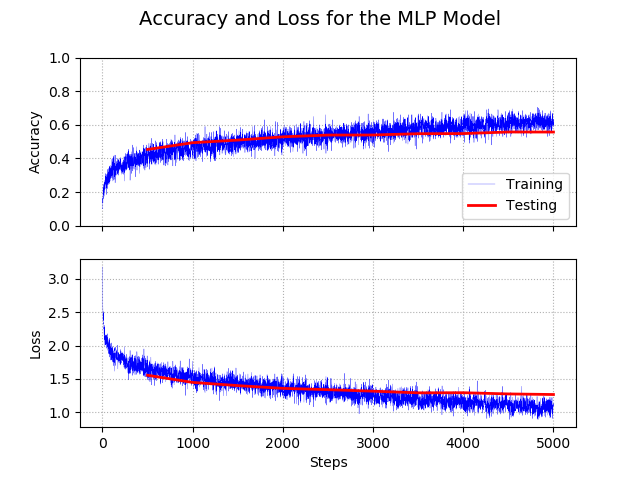
\includegraphics[scale=0.7]{img/mlp_results.png}
    \caption{Training and test accuracies and losses for the MLP model. The test accuracies and losses are produced every 500 steps. The final test accuracy was $55.7 \%$}
    \label{fig:mlp_results}
\end{figure}

% ########################### NEW SECTION ###########################
\section{Custom Module: Batch Normalization}

\subsection{Automatic differentiation}

The automatic differentiation of the batch normalization was implemented as indicated in the code and in the report.

By applying the resulting batch normalization layer after each hidden layer in the MLP model, the test accuracy increased to $57.1 \%$. The loss also decreased to $1.249$. The training curves are shown in Figure \ref{fig:mlp_batchnorm_results}.

\begin{figure}[h]
    \centering
    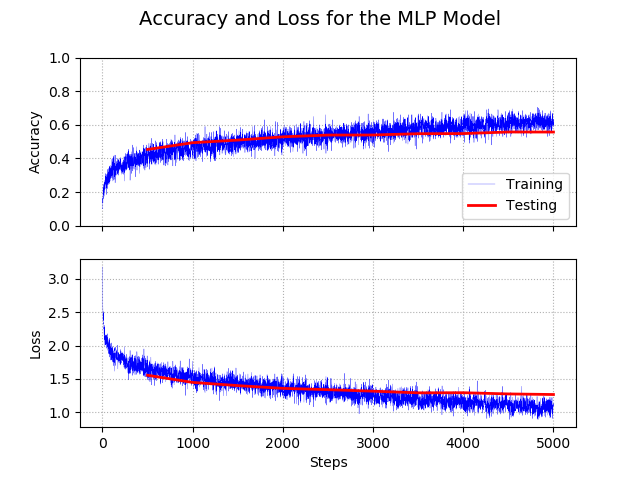
\includegraphics[scale=0.7]{img/mlp_results.png}
    \caption{Training and test accuracies and losses for the MLP model using batch normalization. The test accuracies and losses are produced every 500 steps. The final test accuracy was $57.1 \%$}
    \label{fig:mlp_batchnorm_results}
\end{figure}

\subsection{Manual implementation of backward pass}

I did not have time to do this part of the assignment.

% \subsubsection{}
%
% \subsubsection{}
%
% \subsubsection{}

% ########################### NEW SECTION ###########################
\section{PyTorch CNN}

The training and test accuracies and losses are shown in Figure \ref{fig:convnet_results}.

\begin{figure}[h]
    \centering
    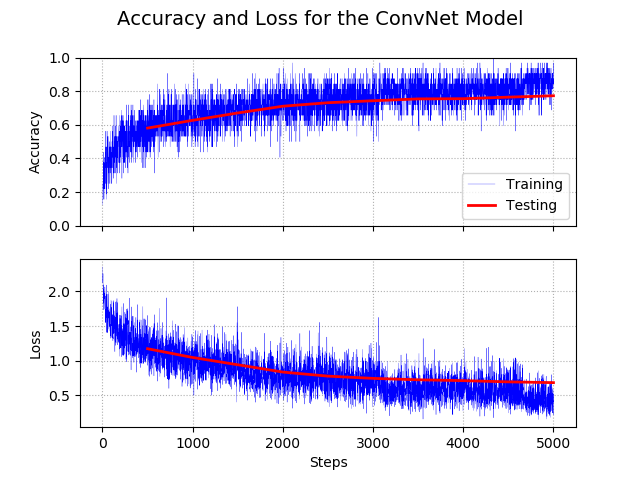
\includegraphics[scale=0.7]{img/convnet_results.png}
    \caption{Training and test accuracies and losses for the ConvNet model. The test accuracies and losses are produced every 500 steps. The final test accuracy was $77.3\%$}
    \label{fig:convnet_results}
\end{figure}

By looking at the plot, we can see that by the end of the training, the network has overfitted on the training data. This occurs around step 3000, which is approximately where the training accuracy becomes higher than the testing accuracy -- and, conversely, where the training loss becomes lower than the testing loss.

The test accuracy measured in the final epoch is $77.3\%$, while the final test loss is $0.681$.

\end{document}
